\documentclass[a4paper, 12pt]{article}

\def\languages{french, english}

%%%%%%%%%%%%%%%%%%% Libraries

%%%%%%%%%% Packages

\usepackage[
backend=biber,
style=numeric-comp,
sorting=none,
maxbibnames=99
]{biblatex}

\newgeometry{margin = 2.5cm}
\makeatletter
\begin{titlepage}
	\begin{minipage}[t][0.425\textheight][t]{\textwidth}
		\begin{center}
		    \ifx\toptitle\undefined
    		    \vfill
    		    \ifx\logopath\undefined
    		    \else
    			    \includegraphics[height=0.2125\textheight]{\logopath}
    			\fi
    		\else
    		    \ifx\logopath\undefined
    		    \else
    			    \includegraphics[height=0.15\textheight]{\logopath}
    			\fi
    			\vfill
    			{\huge \textsc{\toptitle}}
			\fi
			\vfill
		\end{center}
	\end{minipage}
	\vfill
	\begin{minipage}{\textwidth}
		\hspace{0.5em}
		\begin{mdframed}[linewidth = 2pt, innertopmargin = 1em, innerbottommargin = 1em, leftline = false, rightline = false]
			\begin{center}
				{\huge \bfseries \@title}
			\end{center}
		\end{mdframed}
		\hspace{0.5em}
	\end{minipage}
	\vfill
	\begin{minipage}[b][0.425\textheight][t]{\textwidth}
			\ifx\subtitle\undefined
			\else
			    \vspace{-0.5em}
			    \begin{center}
				    {\LARGE \subtitle}
				\end{center}
			\fi
			\vfill
			\ifx\rightauthor\undefined
			    \begin{center}
			        \ifx\authorhead\undefined
			        \else
		                {\large\it \authorhead\\[0.5em]}
		            \fi
			        {\large \@author}
			    \end{center}
			\else
			    \begin{minipage}[t]{0.5\textwidth}
			        \begin{flushleft}
			            \ifx\authorhead\undefined
			            \else
			                {\large\it \authorhead\\[0.5em]}
			            \fi
				        {\large \@author}
				    \end{flushleft}
				\end{minipage}
				\begin{minipage}[t]{0.5\textwidth}
				    \begin{flushright}
				        \ifx\rightauthorhead\undefined
			            \else
			                {\large\it \rightauthorhead\\[0.5em]}
			            \fi
				        {\large \rightauthor}
				    \end{flushright}
				\end{minipage}
			\fi
			\vfill
			\begin{center}
			    \ifx\context\undefined
			    \else
			        {\large \context \\[0.5em]}
			    \fi
			    {\large \@date}
			\end{center}
	\end{minipage}
\end{titlepage}
\makeatother
\restoregeometry
%%%%%%%%%% Packages

\usepackage{float}
\usepackage[skip=1em]{caption}
\usepackage{subcaption}

\usepackage{array}
\usepackage{multirow}
\usepackage{multicol}

%%%%%%%%%% Features

%%%%% Settings

\renewcommand{\arraystretch}{1.2}

%%%%% Commands

\newcommand\noskipcaption[1]{\caption{#1}\vspace{-1em}}
\newcommand\noskipcaptionstar[1]{\caption*{#1}\vspace{-1em}}

%%%%%%%%%% Packages

\usepackage{inconsolata}
\usepackage{listings}

%%%%%%%%%% Features

%%%%% Commands

\newcommand{\Nstyle}[1]{
    \lstdefinestyle{N#1}{
        style=#1,
        %%%%%
        numbers=left
    }
}

\newcommand{\tbFstyle}[1]{
    \lstdefinestyle{tbF#1}{
        style=#1,
        %%%%%
        frame=tb
    }
}

\newcommand{\Fstyle}[1]{
    \lstdefinestyle{F#1}{
        style=#1,
        %%%%%
        frame=single,
        framesep=0em,
        rulesep=0em,
        xleftmargin=0.75em,
        xrightmargin=0.75em,
        framexleftmargin=0.75em,
        framexrightmargin=0.75em,
        framextopmargin=0.5em,
        framexbottommargin=0.5em,
        %%%%%
        numbersep=1.25em
    }
}

\newcommand{\NtbFstyle}[1]{
    \tbFstyle{#1}
    \Nstyle{tbF#1}
}

\newcommand{\NFstyle}[1]{
    \Fstyle{#1}
    \lstdefinestyle{NF#1}{
        style=f#1,
        %%%%%
        xleftmargin=2.75em,
        framexleftmargin=2.75em,
        %%%%%
        numbers=left,
        numbersep=1em
    }
}

%%%%% Styles

\lstdefinestyle{default}{
    breaklines=true,
    breakatwhitespace=true,
    columns=fixed,
	extendedchars=true,
    upquote=true,
	tabsize=4,
    %%%%%
    framerule=0.66pt,
    captionpos=b,
	%%%%%
    basicstyle=\footnotesize\ttfamily,
    numberstyle=\footnotesize\ttfamily,
    showstringspaces=false
}
\Nstyle{default}
\NFstyle{default}
\NtbFstyle{default}

\lstdefinestyle{monokai}{
    style=Fdefault,
    %%%%%
    backgroundcolor=\color[HTML]{272822},
    framerule=0em,
    %%%%%
    basicstyle=\footnotesize\ttfamily\color[HTML]{f8f8f2},
    numberstyle=\footnotesize\ttfamily\color[HTML]{272822},
    commentstyle=\color[HTML]{75715e},
    keywordstyle=[1]{\color[HTML]{f92672}},
    keywordstyle=[2]{\color[HTML]{A6E22E}},
    keywordstyle=[3]{\color[HTML]{ae81ff}},
    stringstyle=\color[HTML]{e6db74},
    %%%%%
    % otherkeywords={!,.,+,-,*,/,=,<,>,^,|,\&,OR,AND}
}

\lstdefinestyle{Nmonokai}{
    style=monokai,
    %%%%%
    xleftmargin=2.75em,
    framexleftmargin=2.75em,
    %%%%%
    numbers=left,
    numberstyle=\footnotesize\ttfamily\color[HTML]{f8f8f2},
    numbersep=1em
}

\lstdefinestyle{c}{
    language=C,
    style=default,
    %%%%%
    commentstyle=\color[HTML]{228B22},
    keywordstyle=\color[HTML]{0000FF},
    stringstyle=\color[HTML]{A020F0},
    emphstyle=\color[HTML]{0000FF},
    %%%%%
    emph={}
}

\lstdefinestyle{cpp}{
    language=C++,
    style=default,
    %%%%%
    commentstyle=\color[HTML]{228B22},
    keywordstyle=\color[HTML]{0000FF},
    stringstyle=\color[HTML]{A020F0},
    emphstyle=\color[HTML]{0000FF},
    %%%%%
    emph={std}
}

\lstdefinestyle{matlab}{
    language=matlab,
    style=default,
    %%%%%
    basicstyle=\footnotesize\fontfamily{pcr}\selectfont,
    numberstyle=\footnotesize\fontfamily{pcr}\selectfont,
    commentstyle=\color[HTML]{228B22},
    keywordstyle=\color[HTML]{0000FF},
    stringstyle=\color[HTML]{A020F0},
    emphstyle=\color[HTML]{0000FF},
    %%%%%
    emph={clearvars}
}

\lstdefinestyle{python}{
    language=python,
    style=default,
    %%%%%
    commentstyle=\color[RGB]{221,0,0},
    keywordstyle=[1]{\color[RGB]{255,119,0}},
    keywordstyle=[2]{\color[RGB]{144,0,144}},
    stringstyle=\color[RGB]{0,170,0},
    emphstyle=\color[RGB]{255,119,0},
    %%%%%
    emph={}
}

\lstdefinestyle{java}{
    language=java,
    style=default,
    %%%%%
    commentstyle=\color[HTML]{228B22},
    keywordstyle=\color[HTML]{0000FF},
    stringstyle=\color[HTML]{A020F0},
    emphstyle=\color[HTML]{0000FF},
    %%%%%
    emph={}
}

%%%%%%%%%% Packages

\usepackage{amsmath}
\usepackage{amssymb}
\usepackage{bm}
\usepackage{esint}
\usepackage[makeroom]{cancel}

%%%%%%%%%% Features

%%%%% Macros

\newcommand{\rbk}[1]{\left(#1\right)}
\newcommand{\cbk}[1]{\left\{#1\right\}}
\newcommand{\sbk}[1]{\left[#1\right]}
\newcommand{\abs}[1]{\left|#1\right|}
\newcommand{\norm}[1]{\left\|#1\right\|}

\newcommand{\fact}[1]{#1!}
\newcommand{\e}[1]{\mathbf{e}_{#1}}
\newcommand{\deriv}{\mathrm{d}}
\DeclareMathOperator{\tr}{tr}

\def\Rl{\mathbb{R}}
\def\Cx{\mathbb{C}}
\def\Na{\mathbb{N}}
\def\Zi{\mathbb{Z}}

%%%%%%%%%% Packages

\usepackage{amsthm}
\usepackage{thmtools}

%%%%%%%%%% Features

%%%%% Settings

\makeatletter
\define@key{thmdef}{mdthm}[{}]{
	\thmt@trytwice{\def\thmt@theoremdefiner{\mdtheorem[#1]}}{}}
\makeatother

\begingroup
\makeatletter
\@for\theoremstyle:=plain,definition,remark\do{
	\expandafter\g@addto@macro\csname th@\theoremstyle\endcsname{
		\addtolength\thm@preskip\parskip
	}
}
\endgroup

\renewcommand{\qedsymbol}{$\blacksquare$}

% language

\ifx\lgthm\undefined
	\def\lgthm{Theorem}
	\def\lgprf{Proof}
	\def\lglem{Lemma}
	\def\lgprop{Proposition}
	\def\lgdefn{Definition}
	\def\lghyp{Hypothesis}
	\def\lgmeth{Method}
	\def\lgquest{Question}
	\def\lgansw{Answer}
	\def\lgexpl{Example}
	\def\lgrmk{Remark}
	\def\lgnote{Note}
	\def\lgtip{Tip}
\fi

%%%%% Commands

\newcommand\qedadd{\pushQED{\qed}\popQED}

%%%%% Environments

\theoremstyle{plain}
\newtheorem{thm}{\lgthm}
\newtheorem{lem}[thm]{\lglem}
\newtheorem{prop}[thm]{\lgprop}

\theoremstyle{definition}
\newtheorem{defn}{\lgdefn}
\newtheorem{hyp}{\lghyp}
\newtheorem{meth}{\lgmeth}
\newtheorem{quest}{\lgquest}

\theoremstyle{remark}
\newtheorem{answ}{\lgansw}[quest]
\newtheorem{expl}{\lgexpl}
\newtheorem*{rmk}{\lgrmk}
\newtheorem*{note}{\lgnote}
\newtheorem*{tip}{\lgtip}

% framed

\mdfdefinestyle{thicc}{
	nobreak=true,
	skipabove=\topskip,
	skipbelow=\topskip,
	innerleftmargin=0.5em,
	innerrightmargin=0.5em,
	innerbottommargin=0.5em,
	innertopmargin=0.5em,
	linewidth=0.25em,
	roundcorner=0.15em,
	linecolor=black!10,
	frametitlebackgroundcolor=black!10,
	theoremseparator={.}
}

\declaretheorem[mdthm={style=thicc, linecolor=red!20, frametitlebackgroundcolor=red!20}, sibling=thm, name=\lgthm]{framedthm}
\declaretheorem[mdthm={style=thicc, linecolor=red!20, frametitlebackgroundcolor=red!20}, sibling=thm, name=\lglem]{framedlem}
\declaretheorem[mdthm={style=thicc, linecolor=blue!20, frametitlebackgroundcolor=blue!20}, sibling=thm, name=\lgprop]{framedprop}
\declaretheorem[mdthm={style=thicc, nobreak=false}, parent=thm, name=\lgprf]{framedprf}

\declaretheorem[mdthm={style=thicc, linecolor=black!20!green!20, frametitlebackgroundcolor=black!20!green!20}, sibling=defn, name=\lgdefn]{frameddefn}
\declaretheorem[mdthm={style=thicc, linecolor=blue!20, frametitlebackgroundcolor=blue!20}, sibling=hyp, name=\lghyp]{framedhyp}
\declaretheorem[mdthm={style=thicc}, name=\lgmeth]{framedmeth}
\declaretheorem[mdthm={style=thicc, linecolor=orange!20, frametitlebackgroundcolor=orange!20}, sibling=quest, name=\lgquest]{framedquest}

\declaretheorem[mdthm={style=thicc, nobreak=false}, sibling=answ, name=\lgansw]{framedansw}
\declaretheorem[mdthm={style=thicc, nobreak=false}, sibling=expl, name=\lgexpl]{framedexpl}

%%%%%%%%%% Packages

\usepackage{siunitx}

%%%%%%%%%% Features

%%%%% Settings

\ifx\decimalsign\undefined
\else
    \sisetup{output-decimal-marker = \decimalsign}
\fi


%%%%%%%%%%%%%%%%%%% Additional packages

\usepackage{bbm}
\usepackage{subcaption}

%%%%%%%%%%%%%%%%%%% Titlepage

\def\logopath{resources/pdf/logo-uliege.pdf}
\def\toptitle{University of Liège}
\title{Bias and variance analysis : Report}
\def\subtitle{Introduction to machine learning}
%\def\authorhead{Author}
\author{
    Maxime \textsc{Meurisse} (20161278)\\
    Valentin \textsc{Vermeylen} (20162864)\\
}
%\def\rightauthorhead{}
%\def\rightauthor{}
\def\context{Master in Civil Engineering, specialization in {\em Intelligent Systems}}
\date{Academic year 2019-2020}

%%%%%%%%%%%%%%%%%%% Options

\geometry{paper=a4paper,top=2.5cm,bottom=2.5cm,right=2cm,left=2cm}
\fancyhead[R]{}
\renewcommand{\thesubsubsection}{(\alph{subsubsection})}

%%%%%%%%%%%%%%%%%%% Document

\begin{document}
    % ----- Titlepage ----- %
    \newgeometry{margin = 2.5cm}
\makeatletter
\begin{titlepage}
	\begin{minipage}[t][0.425\textheight][t]{\textwidth}
		\begin{center}
		    \ifx\toptitle\undefined
    		    \vfill
    		    \ifx\logopath\undefined
    		    \else
    			    \includegraphics[height=0.2125\textheight]{\logopath}
    			\fi
    		\else
    		    \ifx\logopath\undefined
    		    \else
    			    \includegraphics[height=0.15\textheight]{\logopath}
    			\fi
    			\vfill
    			{\huge \textsc{\toptitle}}
			\fi
			\vfill
		\end{center}
	\end{minipage}
	\vfill
	\begin{minipage}{\textwidth}
		\hspace{0.5em}
		\begin{mdframed}[linewidth = 2pt, innertopmargin = 1em, innerbottommargin = 1em, leftline = false, rightline = false]
			\begin{center}
				{\huge \bfseries \@title}
			\end{center}
		\end{mdframed}
		\hspace{0.5em}
	\end{minipage}
	\vfill
	\begin{minipage}[b][0.425\textheight][t]{\textwidth}
			\ifx\subtitle\undefined
			\else
			    \vspace{-0.5em}
			    \begin{center}
				    {\LARGE \subtitle}
				\end{center}
			\fi
			\vfill
			\ifx\rightauthor\undefined
			    \begin{center}
			        \ifx\authorhead\undefined
			        \else
		                {\large\it \authorhead\\[0.5em]}
		            \fi
			        {\large \@author}
			    \end{center}
			\else
			    \begin{minipage}[t]{0.5\textwidth}
			        \begin{flushleft}
			            \ifx\authorhead\undefined
			            \else
			                {\large\it \authorhead\\[0.5em]}
			            \fi
				        {\large \@author}
				    \end{flushleft}
				\end{minipage}
				\begin{minipage}[t]{0.5\textwidth}
				    \begin{flushright}
				        \ifx\rightauthorhead\undefined
			            \else
			                {\large\it \rightauthorhead\\[0.5em]}
			            \fi
				        {\large \rightauthor}
				    \end{flushright}
				\end{minipage}
			\fi
			\vfill
			\begin{center}
			    \ifx\context\undefined
			    \else
			        {\large \context \\[0.5em]}
			    \fi
			    {\large \@date}
			\end{center}
	\end{minipage}
\end{titlepage}
\makeatother
\restoregeometry
    
    % ----- Bayes model and residual error in classification ----- %
    % ----- Q1 ----- %
\section{Bayes model and residual error in classification}

% ----- Q1.a
\subsubsection{{\it Analytical formulation of the Bayes model}}
The zero-one error loss can be written :
$$
L(h_b(x_0, x_1), y) = 1 - \mathbbm{1}_{\{y\}}(h_b(x_0, x_1)) = \begin{cases}
    0 \quad \text{if }h_b(x_0, x_1) = y\\
    1 \quad \text{otherwise} \\
\end{cases}
$$ 
Let's now derive $h_b(x_0, x_1)$ based on the information of the brief.\par
The model being a Bayesian one :
\begin{align*}
    h_b(x_0, x_1) &= \underset{y_i}{\mathrm{argmax}}\ P(y_i | x_0, x_1)\\
    &= \underset{y_i}{\mathrm{argmax}}\ \dfrac{p(x_0, x_1 | y_i) P(y_i)}{p(x_0, x_1)}
\end{align*}
As the class is selected uniformly, $P(y_i) = \num{0.5}$, it is thus constant (independent on the class $y_i$) and we can remove it from the argmax. $p(x_0, x_1)$ also doesn't depend on $y_i$, so we can remove it too. We have :
\begin{align*}
    h_b(x_0, x_1) &= \underset{y_i}{\mathrm{argmax}}\ p(x_0, x_1 | y_i)\\
    &= \begin{cases}
        +1 \quad \text{if }p(x_0, x_1 | y=+1) > p(x_0, x_1 | y=-1)\\
        -1 \quad \text{otherwise}
    \end{cases}
\end{align*}
Let's study the condition for which $h_b(x_0, x_1) = 1$ :
$$
\begin{array}{ccc}
    p(x_0, x_1 | y=+1) & > &  p(x_0, x_1 | y=-1) \\
\end{array}
$$
We need to express $p(x_0, x_1)$ in terms of $p(\alpha)$ and $p(r)$. That method has been provided to us in Stochastic class. The joint probability density of two random variables $X_0 = g_0(r, \alpha)$ and $X_1 = g_1(r, \alpha)$ is :
$$
p_{X_0, X_1}(x_0, x_1) = \dfrac{p_{r, \alpha}(r^{(1)}, \alpha^{(1)})}{|J(r^{(1)}, \alpha^{(1)})|} + ... + \dfrac{p_{r, \alpha}(r^{(k)}, \alpha^{(k)})}{|J(r^{(k)}, \alpha^{(k)})|}
$$
where the $(r^{(1)}, \alpha^{(1)})...(r^{(k)}, \alpha^{(k)})$ are the $k$ roots of the system : 
$$
\begin{cases}
    g_0(r^{(i)}, \alpha^{(i)}) = x_0 \\
    g_1(r^{(i)}, \alpha^{(i)}) = x_1
\end{cases}
$$
and where
$$
J(r^{(i)}, \alpha^{(i)}) = \text{det}\begin{pmatrix}
    \frac{\partial g_0}{\partial r} & \frac{\partial g_0}{\partial \alpha} \\
    \frac{\partial g_1}{\partial r} & \frac{\partial g_1}{\partial \alpha}
\end{pmatrix}
$$
In our case, we have :
$$
\begin{cases}
    x_0 = r \cos{\alpha}\\
    x_1 = r \sin{\alpha}
\end{cases}
$$
and the root of that system is $r^{(1)} = \sqrt{x_0^2 + x_1^2}$, $\alpha^{(1)} = \arctan(\frac{x_1}{x_0})$, with $r > 0$ and $\alpha \in [0, 2\pi[$.
\paragraph{Remark} We only consider the positive $r$, and thus positive $R^+$ and $R^-$. Indeed, the problem is left unchanged, as neglecting the case of negative $r$ associates them with other pairs of $x_0, x_1$. By symmetry, the probabilities are unchanged and the problem stays the same. The ranges of $r$ and $\alpha$ given above ensure a bijection between the two spaces.\par
The Jacobian of our transformation is : 
\begin{align*}
    J(r^{(1)}, \alpha^{(1)}) &= \text{det}\begin{pmatrix}
        \frac{\partial g_0}{\partial r} & \frac{\partial g_0}{\partial \alpha}\\
        \frac{\partial g_1}{\partial r} & \frac{\partial g_1}{\partial \alpha}
    \end{pmatrix} \bigg\rvert_{r^{(1)}, \alpha^{(1)}}\\
    &= \text{det}\begin{pmatrix}
        \cos{\alpha} & -r\sin{\alpha}\\
        \sin{\alpha} & r\cos{\alpha}
    \end{pmatrix}\bigg\rvert_{r^{(1)}, \alpha^{(1)}}\\
    &= r^{(1)} = \sqrt{x_0^2 + x_1^2}\\
\end{align*}
which means that 
$$
p_{X_0, X_1 | y = +1}(x_0, x_1) = \dfrac{p_{r, \alpha | y = +1}(\sqrt{x_0^2 + x_1^2}, \arctan(\frac{x_1}{x_0}))}{\sqrt{x_0^2 + x_1^2}}
$$
and the same is true for the negative class (which only influences the distribution of $r$, not that of $\alpha$). We can safely assume that $p_{r, \alpha} = p_r p_\alpha$ because the two variables are independent, as $\alpha$ is uniformly distributed independently of $y$.\par
We can therefore rewrite our condition for $h_b(x_0, x_1) = 1$ :
$$
\begin{array}{cccc}
    & p(x_0, x_1 | y=+1) & > &  p(x_0, x_1 | y=-1) \\
    \iff & \dfrac{p_{r, \alpha | y = +1}(\sqrt{x_0^2 + x_1^2}, \arctan(\frac{x_1}{x_0}))}{\sqrt{x_0^2 + x_1^2}} & > & \dfrac{p_{r, \alpha | y = -1}(\sqrt{x_0^2 + x_1^2}, \arctan(\frac{x_1}{x_0}))}{\sqrt{x_0^2 + x_1^2}}\\
   \iff & p_{r| y = +1}(\sqrt{x_0^2 + x_1^2})\ p_{\alpha | y = +1}(\arctan(\frac{x_1}{x_0})) & > & p_{r| y = -1}(\sqrt{x_0^2 + x_1^2})\ p_{\alpha | y = -1}(\arctan(\frac{x_1}{x_0}))
\end{array}
$$
As $\alpha$ is independent on $y$ and uniformly distributed, we can remove its probability from the inequality, as it is identical for both sides.\par
The condition therefore writes :
$$
\begin{array}{cccc}
    & p_{r| y = +1}(\sqrt{x_0^2 + x_1^2}) & > & p_{r| y = -1}(\sqrt{x_0^2 + x_1^2})\\
    \iff & \dfrac{1}{\sqrt{2\pi\sigma^2}}\exp{-\dfrac{(\sqrt{x_0^2 + x_1^2} - R^+)^2}{2\sigma^2}} & > & \dfrac{1}{\sqrt{2\pi\sigma^2}}\exp{-\dfrac{(\sqrt{x_0^2 + x_1^2} - R^-)^2}{2\sigma^2}}\\
    \iff & \exp{-\dfrac{(\sqrt{x_0^2 + x_1^2} - R^+)^2}{2\sigma^2}} & > & \exp{-\dfrac{(\sqrt{x_0^2 + x_1^2} - R^-)^2}{2\sigma^2}}\\
    \iff & -\dfrac{(\sqrt{x_0^2 + x_1^2} - R^+)^2}{2\sigma^2} & > & -\dfrac{(\sqrt{x_0^2 + x_1^2} - R^-)^2}{2\sigma^2}\\
\end{array}
$$
The last step coming from the fact that the exponential is a monotonic increasing function, so a greater argument implies a greater value of the function and vice-versa.\par
By removing the denominator and arranging the terms, we finally have : 
$$
\begin{array}{cccc}
   &  \dfrac{(\sqrt{x_0^2 + x_1^2} - R^+)^2}{2\sigma^2} & < & \dfrac{(\sqrt{x_0^2 + x_1^2} - R^-)^2}{2\sigma^2}\\
   \iff & (\sqrt{x_0^2 + x_1^2} - R^+)^2 & < & (\sqrt{x_0^2 + x_1^2} - R^-)^2\\
   \iff & 2\sqrt{x_0^2 + x_1^2} (R^--R^+) & < & (R^-)^2 - (R^+)^2\\
   \iff & \sqrt{x_0^2 + x_1^2} & > & \dfrac{R^- + R^+}{2}
\end{array}
$$
It has to be noted that we have assume that $R^-$ is smaller than $R^+$. If it is not the case, the decision process simply has to be inverted, as the inequality sign change is not applicable.\par
In the end, we have : 
$$
h_b(x_0, x_1) = \begin{cases}
    +1 \quad \text{if }\sqrt{x_0^2 + x_1^2}  > \dfrac{R^- + R^+}{2}\\
    -1 \quad \text{otherwise}\\
\end{cases}
$$
if $R^- < R^+$. If $R^- > R^+$, the conclusion simply has to be inverted. We do not discuss the case $R^- = R^+$ as the inputs would be independent of the output, and no prediction could be made on the basis of their values. 

% ----- Q1.b
\subsubsection{{\it Analytical formulation of the residual error}}
The prediction of our Bayes model depending only on $r$, let's calculate the error as follow, as $\alpha$ is not taken into account for the prediction, and therefore does not impact the error :
$$
E_{x_{0}, x_{1}, y}\left\{1\left(y \neq h_{b}\left(x_{0}, x_{1}\right)\right)\right\} = E_{r, y}\left\{1\left(y \neq h_{b}\left(r\right)\right)\right\}
$$
As we are in classification, the generalization of the zero-one loss function is equivalent to the probability of wrongly predicting the output based on the input :
\begin{align*}
    E_{r,y}\left\{1\left(y \neq h_{b}\left(x_{0}, x_{1}\right)\right)\right\} &= P(y = +1, h_b(r) = -1) + P(y = -1, h_b(r) = +1)\\
    &= P(h_b(r) = -1 | y = +1)P(y = +1) + P(h_b(r) = +1 | y = -1)P(y = -1)\\
    &= \frac{1}{2}P(h_b(r) = -1 | y = +1) + \frac{1}{2}P(h_b(r) = +1 | y = -1)
\end{align*}
via the Bayes theorem and because $P(y = y_i) = 0.5$. We have that : 
$$
P(h_b(r) = -1 | y = +1) = \int_{0}^{\dfrac{R^+ + R^-}{2}} \dfrac{1}{\sqrt{2\pi\sigma^2}} \exp{-\dfrac{(r - R^+)^2}{2\sigma^2}} dr
$$
and
$$
P(h_b(r) = +1 | y = -1) = \int_{\dfrac{R^+ + R^-}{2}}^{+\infty} \dfrac{1}{\sqrt{2\pi\sigma^2}} \exp{-\dfrac{(r - R^-)^2}{2\sigma^2}} dr
$$
By replacing these probabilities by their analytical forms in the generalization error, we have an analytical formulation of the error which is hard to compute by hand. By replacing the values of $R^+$, $R^-$ and $\sigma$ from what is given in the brief and using \href{https://www.wolframalpha.com}{WolframAlpha} to solve it, we have that the error is equal to :
$$
E_{r, y}\left\{1\left(y \neq h_{b}\left(r\right)\right)\right\} = 0.5 * 0.0569231 + 0.5 * 0.0569231 = 0.0569231 \approx 5.7\%
$$
\paragraph{Remark} Had we had to compute the integrals by hand, we could either have used the error function $erf$ or the Gaussian random variable distribution tables seen in probability class (and we would have to normalize the distribution of $r$ to do so).

    
    % ----- Bias and variance of the kNN algorithm ----- %
    \newpage
    % ----- Q2 ----- %
\section{Bias and variance of the kNN algorithm}

% ----- Q2.a
\subsubsection{{\it Decomposition of the generalization error}}
From the slide 12 of the lesson 6, we have that the generalization error decomposition is the following :
$$
E_{L S}\left\{E_{y}\left\{(y-\hat{y})^{2}\right\}\right\} = E_{y}\left\{\left(y-E_{y}\{y\}\right)^{2}\right\} + E_{L S}\left\{\left(E_{y}\{y\}-\hat{y}\right)^{2}\right\}
$$
and, from the slide 14, we get that : 
$$
E_{L S}\left\{\left(E_{y}\{y\}-\hat{y}\right)^{2}\right\} = \left(E_{y}\{y\}-E_{L S}\{\hat{y}\}\right)^{2}+E_{L S}\left\{\left(\hat{y}-E_{L S}\{\hat{y}\}\right)^{2}\right\}
$$
where
\begin{align*}
    E_{y}\left\{\left(y-E_{y}\{y\}\right)^{2}\right\} &= \text{var}_y\{y\}\\
    \left(E_{y}\{y\}-E_{L S}\{\hat{y}\}\right)^{2} &= \text{bias}^2\\
    E_{L S}\left\{\left(\hat{y}-E_{L S}\{\hat{y}\}\right)^{2}\right\} &= \text{var}_{LS}\{\hat{y}\}
\end{align*}
However, what we want is to find a function $\hat{y}(\mathbf{x})$ of several inputs, and so we average over the whole input space. For one learning set, the error becomes $E_{\mathbf{x}, y}\left\{(y-\hat{y}(\mathbf{x}))^{2}\right\}$. Over all the learning sets, we have that the error writes : 
\begin{align*}
    E &= E_{L S}\left\{E_{\mathbf{x}, y}\left\{(y-\hat{y}(\mathbf{x}))^{2}\right\}\right\}\\
    &= E_{\mathbf{x}}\left\{E_{L S}\left\{E_{y | \mathbf{x}}\left\{\left(y-\hat{y}((x))^{2}\right\}\right\}\right\}\right.\\
    &= E_{\mathbf{x}}\left\{\operatorname{var}_{y | \mathbf{x}}\{y\}\right\}+E_{\mathbf{x}}\left\{\operatorname{bias}^{2}(\mathbf{x})\right\}+E_{\mathbf{x}}\left\{\operatorname{var}_{L S}\{\hat{y}(\mathbf{x})\}\right\}
\end{align*}
\paragraph{Remark} This is taken from the slide 21.\par
Finally, from the slide 22 (which derives an equality from the two last lines of the error decomposition above) we have that :
\begin{align*}
    E_{L S}\left\{E_{y | \mathbf{x}}\left\{(y-\hat{y}(\mathbf{x} ; L S, k))^{2}\right\}\right\} &= E_{y | \mathbf{x}}\left\{\left(y-h_{B}(\mathbf{x})\right)^{2}\right\} + \left(h_{B}(\mathbf{x})-E_{L S}\{\hat{y}(\mathbf{x})\}\right)^{2}\\
    &+ E_{L S}\left\{\left(\hat{y}-E_{L S}\{\hat{y}(\mathbf{x})\}\right)^{2}\right\}    
\end{align*}
where $h_{B}(\mathbf{x})=E_{y | \mathbf{x}}\{y\}$.\par
Given $\mathbf{x}$, we know the value of $y = f(\mathbf{x}) + \epsilon$, except for the $\epsilon$ which is a random variable.\par
Therefore,
\begin{align*}
    E_{y | \mathbf{x}}\{y\} &= E\{f(\mathbf{x}) + \epsilon\}\\
    &= E\{f(\mathbf{x})\}\\
    &= f(\mathbf{x})
\end{align*}
because the expected value of a sum is equal to the sum of the expected values, $E\{\epsilon\} = 0$ as the mean of $\epsilon$ is $0$, and the expected value of a constant ($f(\mathbf{x})$) is that constant (as $\mathbf{x}$ is fixed beforehand).\par
Plugging that into the equation (where LHS represents the left-hand side of the said equation), we get :
$$
LHS = E\left\{\left(f(\mathbf{x}) + \epsilon-f(\mathbf{x})\right)^{2}\right\} + \left(f(\mathbf{x})-E_{L S}\{\hat{y}(\mathbf{x})\}\right)^{2} + E_{L S}\left\{\left(\hat{y}-E_{L S}\{\hat{y}(\mathbf{x})\}\right)^{2}\right\}    
$$
We have that
\begin{align*}
    E\left\{\epsilon^{2}\right\} &= \text{var}\{\epsilon\} + E\{\epsilon\}^2\\
    &= \sigma^2 + 0\\
    &= \sigma^2
\end{align*}
via the expansion of the variance and the information we have about $\epsilon$.\par
The last term of the sum is equivalent to the variance of $\hat{y}$ over all datasets, via the definition of the variance.\par
As
\begin{align*}
    \hat{y} &= \frac{1}{k} \sum_{l=1}^k y_{(l)}\\
    &= \frac{1}{k} \sum_{l=1}^k \left(f(\mathbf{x}_{(l)})+\epsilon\right)
\end{align*}
because, for the $kNN$ regression, the estimated value is the average of those of all neighbours. For a given $\mathbf{x}_{(l)}$, the value of $f(\mathbf{x}_{(l)})$ is not a random variable, and is thus a constant.\par
Therefore,
\begin{align*}
    \text{var}_{L S}\left\{ \hat{y} \right\} &= \text{var}_{L S}\left\{ \frac{1}{k} \sum_{l=1}^k \left(f(\mathbf{x}_{(l)})+\epsilon\right) \right\}\\
    &= \frac{1}{k^2} \text{var}_{L S}\left\{\sum_{l=1}^k \left(f(\mathbf{x}_{(l)})+\epsilon\right) \right\}\\
    &= \frac{1}{k^2} \ k\ \text{var}_{L S}\left\{ \epsilon \right\}\\
    &= \dfrac{\sigma^2}{k}
\end{align*}
Because $\text{var}\left\{ a X \right\} = a^2 \text{var}\left\{ X \right\}$, the variance of the sum of independent random variables is the sum of the variances and, finally, because $\text{var}\left\{ X + a \right\} = \text{var}\left\{ X \right\}$, $a$ being a constant here.\par
For the second term,
\begin{align*}
    E_{L S}\left\{\hat{y}(\mathbf{x})\right\} &= E_{L S}\left\{ \frac{1}{k} \sum_{l=1}^k \left(f(\mathbf{x}_{(l)})+\epsilon\right) \right\}\\
    &= \frac{1}{k} E_{L S}\left\{\sum_{l=1}^k \left(f(\mathbf{x}_{(l)})+\epsilon\right) \right\}\\
    &= \frac{1}{k} E_{L S}\left\{\sum_{l=1}^k \left(f(\mathbf{x}_{(l)})\right) \right\}\\
    &= \frac{1}{k} \sum_{l=1}^k \left(f(\mathbf{x}_{(l)})\right)
\end{align*}
Because $E\{aX\} = aE\{X\}$, $E\{A+X\} = E\{A\} + E\{X\}$, $E\{\epsilon\} = 0$ and $E\{f(\mathbf{x}_{(l)})\} = f(\mathbf{x}_{(l)})$ because the argument is a constant.\par
By plugging all these results in the equation, we end up with what is given in the brief.
\begin{comment}
    From the slides of the lecture 6, we have that : 
    $$\begin{array}{ccc}
        E_{L S}\left\{E_{y | \mathbf{x}}\left\{(y-\hat{y}(\mathbf{x} ; L S, k))^{2}\right\}\right\} & = &  var_{y|\mathbf{x}}\left\{y \right\} + \left( E_{y|\mathbf{x}}\left\{y \right\} - E_{LS} \left\{ \hat{y}\right\}\right)^2 +  E_{LS}\left\{ \left( \hat{y} - E_{LS}\left\{ \hat{y}\right\}\right)^2\right\}\\
    \end{array}
    $$
    Given the decomposition seen in class. We also know that $y = f(\mathbf{x}) + \epsilon$. By pushing that into the equation, we have : 
    $$\begin{array}{ccc}
        E_{L S}\left\{E_{y | \mathbf{x}}\left\{(y-\hat{y}(\mathbf{x} ; L S, k))^{2}\right\}\right\} & = &  \sigma_\epsilon^2 + \left( f(\mathbf{x}) - E_{LS} \left\{ \hat{y}\right\}\right)^2 + E_{LS}\left\{ \left( \hat{y} - E_{LS}\left\{ \hat{y}\right\}\right)^2\right\}\\
    \end{array}
    $$
    Because $var_y{f(\mathbf{x}) + \epsilon} = var{\epsilon} = \sigma_\epsilon^2$ as $f(\mathbf{x})$ is a scalar, $E_y \{f(\mathbf{x}) + \epsilon\} = E_y \{f(\mathbf{x})\} = f(\mathbf{x})$ for the same reason, and because the expectation of $\epsilon$ is $0$.
\end{comment}

% ----- Q2.b
\subsubsection{{\it Effect of the number of neighbours}}
As can be seen in the previous decomposition, there is a term, $\sigma^2$, that is not affected by the number of neighbours $k$. That is the \textit{irreductible error}, and it is out of our control, even if we knew the actual $f(\mathbf{x})$. This term comes from the noise $\epsilon$ in the computation of $y$. It is the minimal error possibly atteinable.\par
However, we can control the other two terms. The second is the bias and the third is the variance.\par
The bias term will likely increase with $k$ in the case of this estimator, provided that $f$ is smooth enough. Indeed, for a small $k$, the few closest neighbours will have values of $f(\mathbf{x}_{(l)})$ close to $f(\mathbf{x})$, and so the average of these values itself should be close to $f(\mathbf{x})$, which makes the bias close to $0$.\par
Conversely, as $k$ increases, the neighbours are further away from $\mathbf{x}$, and so anything can happen. The values of $f(\mathbf{x}_{(l)})$ could become much more different from that of $f(\mathbf{x})$ and generate a big bias, or maybe not if $f(\mathbf{x})$ is more constant over the dataset space, but that is usually not the case, and so the bias increases with $k$.\par
For the variance, it decreases as the inverse of $k$, so a big $k$ yields a small variance because we are not basing our decision only on a few close points. As $k$ grows to infinity, the model becomes less complex as we will predict the majority class for all test points. Conversely, with a small $k$, the model will be more sensitive on the training data as its decision will be based on close, specific points that depends more heavily on the specific learning set, and so its variance will increase as a result because two different learning sets will not have identical samples. For a higher number of neighours, that effect is mitigated as we start to encompass a bigger region in our decision process, and so the variance decreases. For bigger regions of the space of inputs, the variance in the sampling for two different datasets will be smaller than for smaller regions, and thus the overall variance decreases.\par
As we can see, there is therefore a tradeoff to be made between bias and variance as the effect of $k$ on each is inverse and as they both play a role in the generalization error.

    
    % ----- Bias and variance estimation ----- %
    \newpage
    % ----- Q3 ----- %
\section{Bias and variance estimation}

% ----- Q3.a
\subsubsection{{\it Protocol for a given point}}\label{Q3.a}
The following protocol is used to estimate the residual error, the squared bias and the variance for a given point $x_0$ and for a supervised learning algorithm.\par
\paragraph{Remark} In the protocol, $x_0$ can refer to a single feature or multiple features. In the case of multiple features, when we talk about comparing $x_0$ to a value, it will be a question of comparing the whole tuple of values to the other tuple.\par
First, since we assume that we can generate an infinite number of samples, we generate a large number of datasets (for example, \num{30}) each containing a large number of samples $(x, y)$ (for example, \num{1000}).\newline
NB : Were we not limited by computational power, we could take an infinite number of datasets containing each an infinite number of samples to estimate these values perfectly.\par
Secondly, we select in each of the datasets all the values of $y$ whose associated $x$ is $x_0$. These values will be represented by $y_{x_0}^{(i)}$.\par
Thirdly, we instantiate one model (always the same) per dataset and we train each model on one of the datasets. Each model is then asked to provide the value associated with $x_0$. These values will be represented by $\hat{y}_{x_0}^{(i)}$.\par
Finally, to estimate the residual error, the variance of $y_{x_0}$ is computed, to estimate the square bias, the difference squared between the mean of $y_{x_0}$ and the mean of $\hat{y}_{x_0}$ is computed and to estimate the variance, the variance of $\hat{y}_{x_0}$ is computed.

% ----- Q3.b
\subsubsection{{\it Adapted protocol}}\label{Q3.b}
The following protocol is used to estimate the mean value of the residual error, squared bias and variance (as defined in section \ref{Q3.a}).\par
First, the protocol described in section \ref{Q3.a} is used to calculate the residual error, squared bias and variance for each point $x_i$ generated in the datasets.\par
Then the average on all $x$ of all residual errors, squared bias and variances obtained is computed and these are the values we need.

% ----- Q3.c
\subsubsection{{\it Case of a finite number of samples}}
The protocols described above will still be usable, however their results may not be reliable.\par
Indeed, if we have a small number of samples, the datasets we create will contain a very small number of data (for example, if we have \num{50} samples, we can create \num{5} datasets of \num{10} samples each). The models will therefore be trained on a very small number of data and will give poor results as there will be a lot of underfitting.\par
If the trained models are not good and their results are not reliable, the residual error, squared bias and variance calculated on the basis of these models will not be reliable and significant either. Furthermore, to apply the protocols, we need to have multiple points that are at the same $x_0$, which cannot happen if we have too small datasets. The protocol \ref{Q3.a} relies almost entirely on the fact that there will be many samples having the same input value $x_0$. If it was not the case, we couldn't compute the desired components of the error in a satisfying manner. For protocol \ref{Q3.b}, we also need to have a lot of samples to accurately approximate the mean values over the input space, otherwise we are too dependent on the dataset itself. To conclude, if we do not have enough values for the same $x_0$ and not enough $x_0$, the protocols are not appropriate anymore. We therefore need lots of sample for our protocols to be appropriate.

% ----- Q3.d
\subsubsection{{\it Application of the protocol}}
The script for this question, applying the protocol described in section \ref{Q3.a}, can be found in file \texttt{Q3d.py} attached to this report.\par
In order to facilitate the recovery of the values of $y$ associated with an $x_i$ value (or tuple of values), only one vector containing the samples of all datasets was generated. This vector is then divided into sub-vectors to train the different models.\par
For this question, we used a dataset of \num{10000} samples which we divided into \num{10} training sets of \num{1000} samples each.\par
All generated samples are shown in figure \ref{fig:Q3d_data}.
\begin{figure}[H]
    \centering
    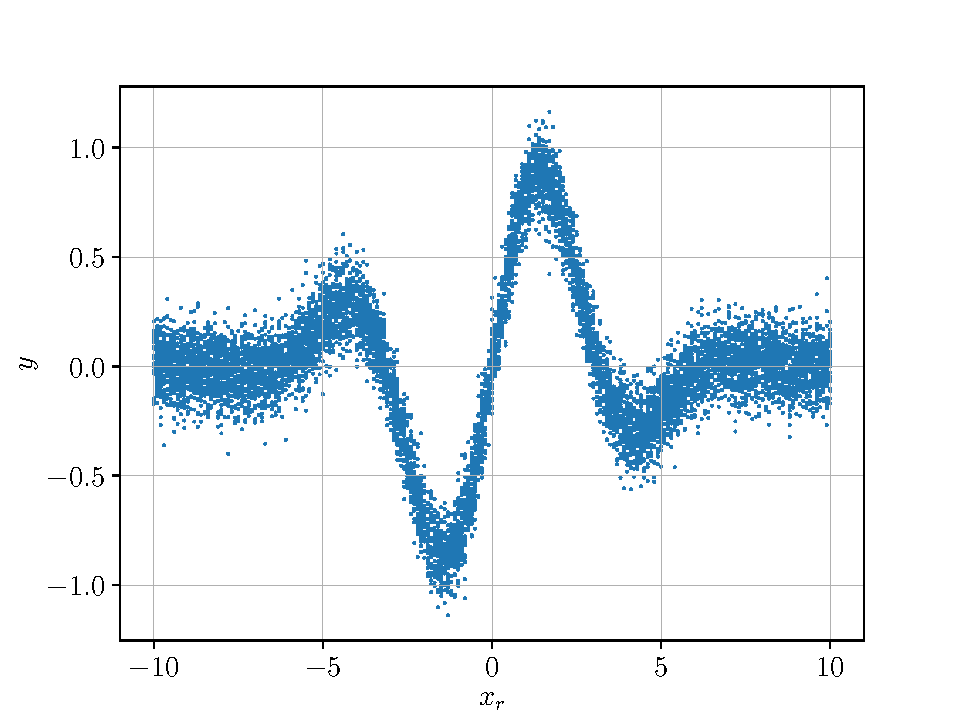
\includegraphics[width=0.8\textwidth]{resources/pdf/Q3d_data.pdf}
    \caption{All generated samples (\num{10000})}
    \label{fig:Q3d_data}
\end{figure}
For {\bf linear regression}, the Ridge algorithm was chosen. For {\bf non linear regression}, the k nearest neighbors regressor was chosen.\par
The residual error, squared bias, variance and expected error as a function of $x$ for both cases are shown in figure \ref{fig:Q3d_error}. In order to facilitate their comparison, all elements are represented on the same figure with a logarithmic scale.
\begin{figure}[H]
    \centering
    \begin{subfigure}{0.495\textwidth}
        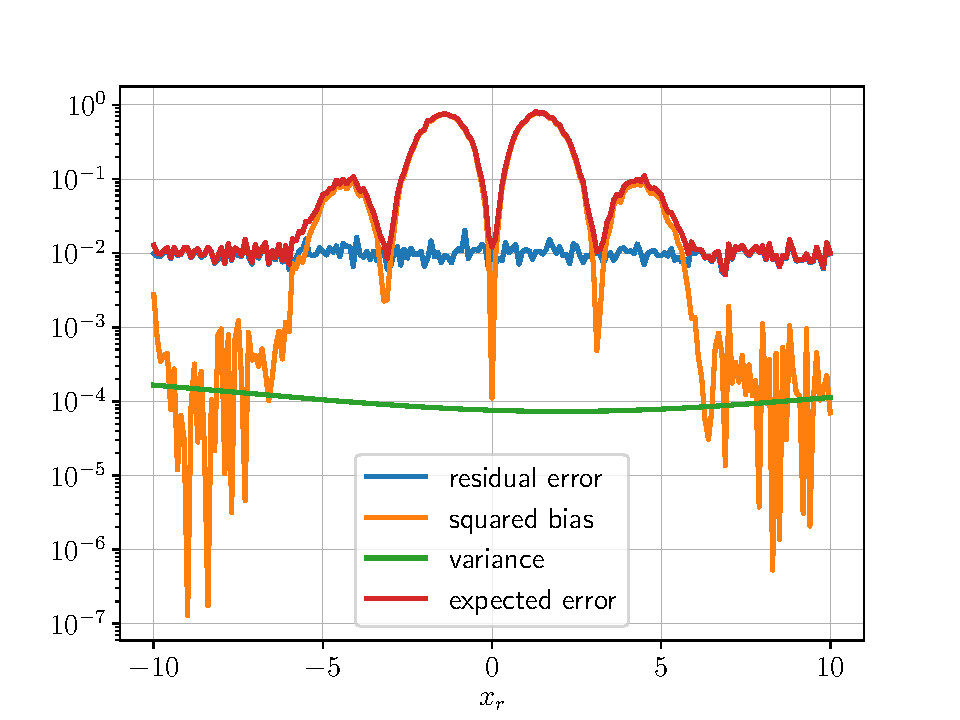
\includegraphics[width=\textwidth]{resources/pdf/Q3d_Ridge.pdf}
        \caption{Ridge regression}
        \label{fig:Q3d_ridge}
    \end{subfigure}
    \begin{subfigure}{0.495\textwidth}
        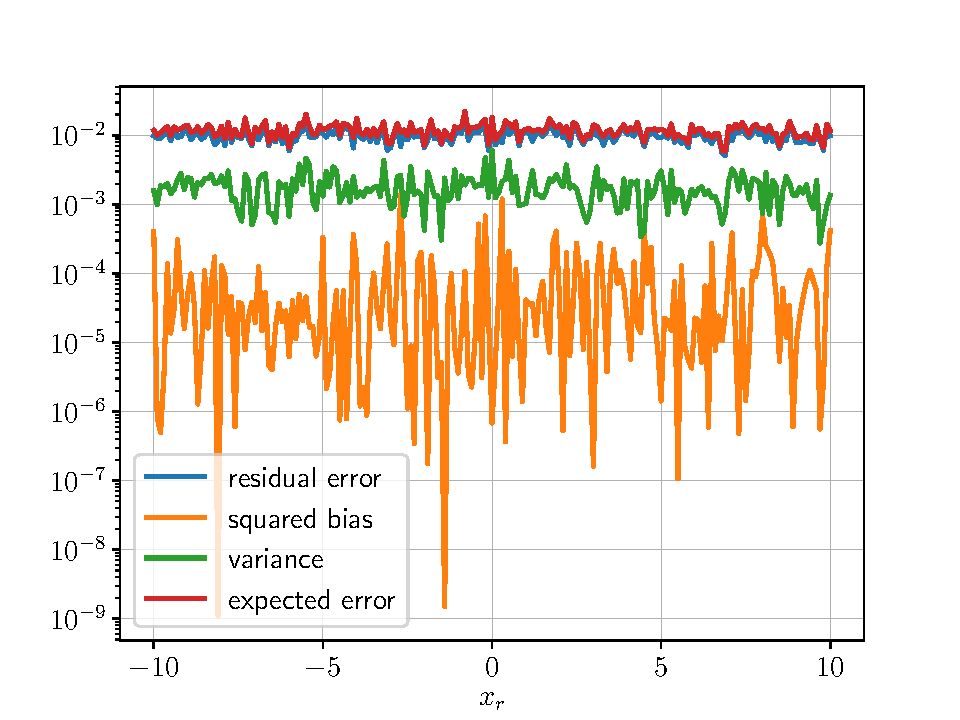
\includegraphics[width=\textwidth]{resources/pdf/Q3d_KNeighborsRegressor.pdf}
        \caption{K neighbors regression}
        \label{fig:Q3d_kneighborsregressor}
    \end{subfigure}
    \noskipcaption{Estimation of the residual error, the squared bias, the variance and the expected error as a function of $x$}
    \label{fig:Q3d_error}
\end{figure}
In the case of {\bf linear regression}, we find that the expected error is quite close to the squared bias. This result seems logical since linear regression is not at all appropriate in this case. Indeed, linear algorithms tend to have a higher bias than non-linear ones, as the simplifying assumptions they make (quasi-linearity of $y$ given $x_r$ here) usually fail to meet the more complex reality, inducing larger errors\footnote{\href{https://machinelearningmastery.com/gentle-introduction-to-the-bias-variance-trade-off-in-machine-learning/}{https://machinelearningmastery.com/gentle-introduction-to-the-bias-variance-trade-off-in-machine-learning/}}.\par
Indeed, it is assumed that the regression obtained is a horizontal curve whose equation must be very similar to $y = 0$ because the distribution is quite \og{}symmetric\fg{} around $y=0$ (the figure is not shown here but it is indeed the shape we obtain when running our codes). As a result, the regression gives good results for samples corresponding to $x_r < -5$ and $x_r > 5$ as their $y$ values are close to $0$, as seen in figure \ref{fig:Q3d_data}. However, between these two values, the regressed line does not approximate well the real curve (the effect of the sinus is more prevalent as it is less dampened for these $x_r$), thus increasing the approximation error.\par
This phenomenon can be observed in figure \ref{fig:Q3d_ridge} : the bias has \num{4} humps, one per sinus oscillation. The two small extreme humps correspond to the two extreme oscillations, and the two large middle humps correspond to the two large oscillations. The bias is greater in these regions because the hypothesis of linearity is more false than on the \og{}sides\fg{}, and so the difference between the value estimated (which is close to $0$) and the real value has roughly the shape of the sine itself, with only negative concavity because the bias is squared.\par
The variance, on the other hand, remains quite low. Being clearly in the presence of under fitting, this observation is logical. Indeed, as we take $1000$ samples in our learning sets, their distribution will not change greatly from one learning set to another, and thus will not greatly impact the predictions. Had we taken a much smaller learning set size, we would have observed a greater variance, as the distributions of the samples would have been more varied from one dataset to another, impacting more the prediction. The variance also seems to be independent of $x_r$, and that is because the algorithm will predict a line close to $y = 0$ for all $x_r$. \par
Finally, the residual error is almost constant as it is independent from the input (it is a Gaussian noise).\par
In the case of {\bf non-linear regression}, it is the residual error that dominates (see figure \ref{fig:Q3d_kneighborsregressor}) given our parameters. Bias and variance are relatively low. These results show us that non-linear regression is better suited to this case, as figure \ref{fig:Q3d_data} suggested. Indeed, KNN works quite well in this situation as we can generate a lot of samples and the training is done on 1000 of them. The value at any given point is the mean of its 5 closest neighbours, and as they are quite close due to the large training set we used, the bias is small. Having training samples that are uniformly distributed and quite dense, we can have really good approximations, but we cannot act on the residual error (it is the smallest possible error we can reach as it is random noise in the output). The variance is also small because we will likely find similar (close) samples for different datasets as we have a high number of training samples. 

% ----- Q3.e
\subsubsection{{\it Application of the protocol for different input variations}}
The script for this question, applying the protocol described in section \ref{Q3.b}, can be found in file \texttt{Q3e.py} attached to this report.\par
The mean values of the squared error, the residual error, the squared bias and the variance for multiple variations of some parameters are described in the following sections. In order to facilitate their comparison, all elements are represented on the same figure with a logarithmic scale.\par
By default, we used 10 training sets of 1000 samples each with 0 irrelevant variable. The default complexity of our models is $\alpha = 1.0$ for Ridge and $n\_neighbors = 5$ for K neighbors regressor.\par
In the following sections, when we vary a quantity, we take the default values of the others.

% Function of the size of the learning set
\subsubsection*{Function of the size of the learning set}
\begin{figure}[H]
    \centering
    \begin{subfigure}{0.495\textwidth}
        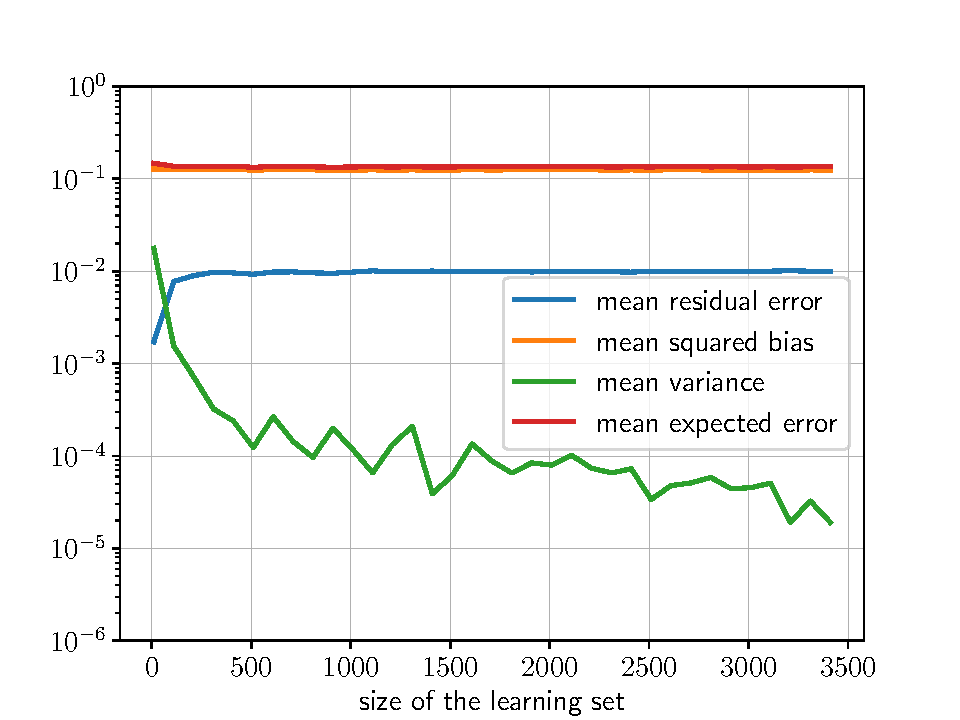
\includegraphics[width=\textwidth]{resources/pdf/Q3e_Ridge_size_ls.pdf}
        \caption{Ridge regression}
    \end{subfigure}
    \begin{subfigure}{0.495\textwidth}
        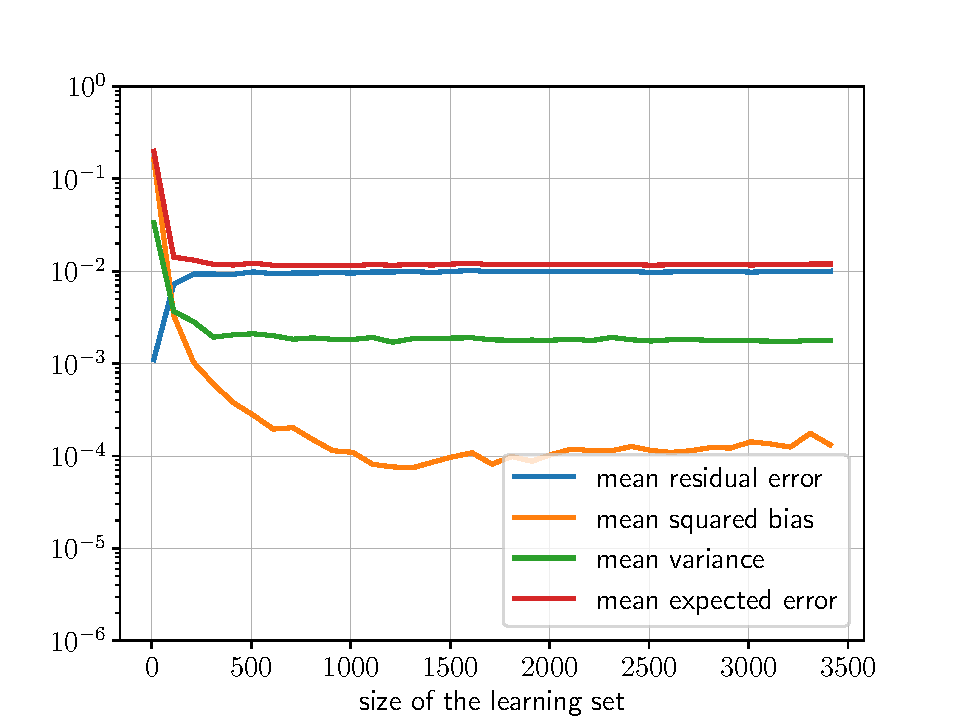
\includegraphics[width=\textwidth]{resources/pdf/Q3e_KNeighborsRegressor_size_ls.pdf}
        \caption{K neighbors regression}
    \end{subfigure}
    \noskipcaption{Mean of the error and its terms as a function of the size of the learning set}
\end{figure}
For both models, it can be seen that the residual error is constant after a given size (although it has been said in Q3c that the protocols are inappropriate for small sizes of the learning set, we still included the beginning). This result is unsurprising because the residual error represents the noise in the data and is normally independent of the size of the dataset. The rise in the beginning comes from the fact that our protocol does not approximate well the different values for small sizes of datasets. It should be dismissed.\par
The squared bias remains constant for the linear model and decreases for the non-linear model up to a given point. This shows that the linear model is not adapted (even if the size of the learning set is increased, the quality of the regression does not improve). As the distribution of $y$ oscillates quite symmetrically around $0$, no matter the number of samples we will take, given that the sampling is uniform on the input space, which is the case, the squared bias will tend to stay the same as the prediction will always be something in the lines of $\hat{y} = 0$ because we will have a roughly symmetrical sampling of values around $y = 0$. This also highlights the fact that the non-linear model is more adapted to that problem (the larger the learning set, the lower the error).\newline
For KNN, the bias is high for small learning sets because the learning samples will be few and the prediction will probably be based on farther, less relevant samples, whereas, for larger datasets, we will find samples that are closer to our point, and so the bias decreases. (However, we can see that, after a given size of about 1000 samples, the mean expected error for KNN does not decrease anymore. Indeed, adding more samples will not change greatly the minimal obtainable error as we already have enough samples that are close enough to the point we try to evaluate.) \par
In both cases, the variance decreases. Indeed, with a small amount of data, the models train on a too restricted vision of the input space leading to poor results and high variance. Specific learning sets lead to highly different results for smaller sizes, and so the variance is high. For larger datasets, the learning samples will always be located roughly at the same positions, and so the predictions will not vary much among the datasets, leading to a smaller variance. The larger the size of the learning set, the better the models will be trained and the more the variance will decrease (up to a given point for KNN as, for very large learning sets, we will have almost always the same-or very similar-points counted as neighbors, and so the variance will not decrease anymore). It is thus unnecessary to have larger learning sets because the variance becomes negligible for the linear regression (and is the only metrics that changes for bigger sizes), and because nothing decreases anymore for KNN.\par

% Function of the model complexity
\subsubsection*{Function of the model complexity}
For the linear model, the complexity is the value of $\alpha$ and, for KNN, it is the number of neighbors.
\begin{figure}[H]
    \centering
    \begin{subfigure}{0.495\textwidth}
        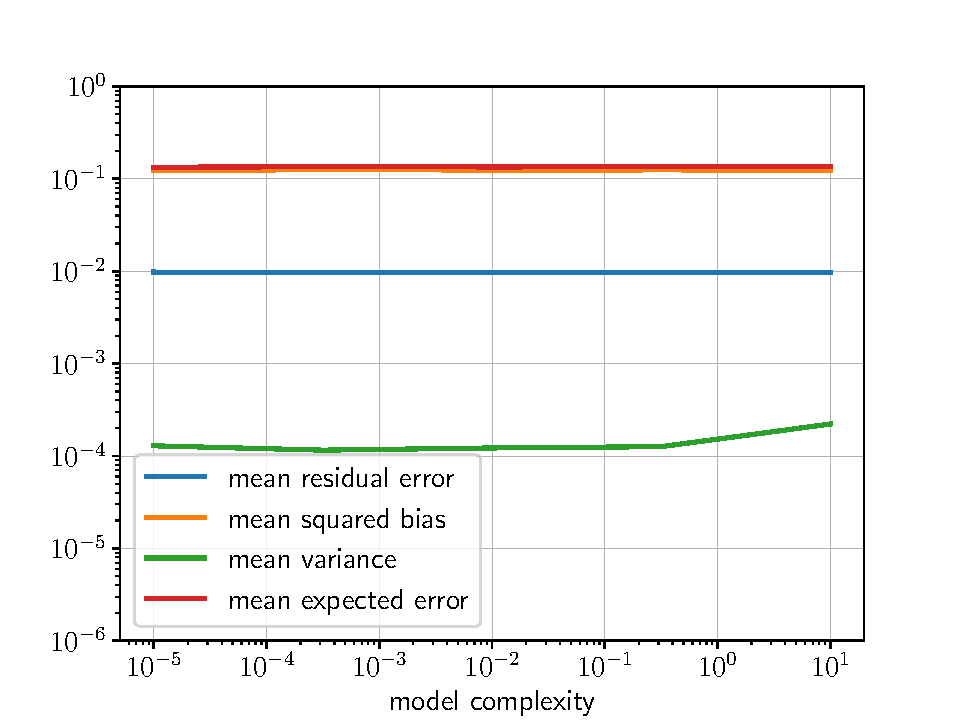
\includegraphics[width=\textwidth]{resources/pdf/Q3e_Ridge_model_complexity.pdf}
        \caption{Ridge regression}
    \end{subfigure}
    \begin{subfigure}{0.495\textwidth}
        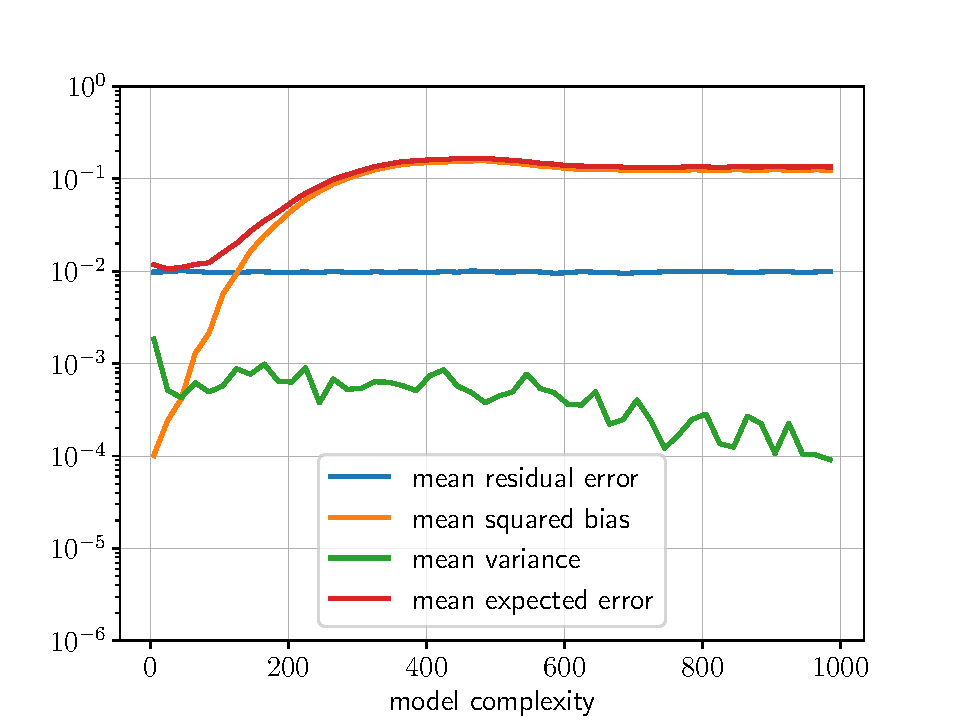
\includegraphics[width=\textwidth]{resources/pdf/Q3e_KNeighborsRegressor_model_complexity.pdf}
        \caption{K neighbors regression}
    \end{subfigure}
    \noskipcaption{Mean of the error and its terms as a function of the model complexity}
\end{figure}
In both cases, as before, the residual error remains constant; it does not depend on the complexity of the model.\par
In the linear model, the expected error is dominated by the squared bias which remains constant and high. Indeed, when we take a look at the learning samples, no matter the value of $\alpha$, the predicted curve will always tend to be close to $y = 0$ as a result of the symmetry of f($\mathbf{x}$). This shows once again that the linear model is not suitable : no matter how complex the model, a big error is made and it does not decrease.\par
In the non-linear model, the squared bias increases a lot with the number of neighbors taken into consideration. It is easily understood as, the more samples you take into account, the more uncorrelated samples are present. To have a small bias, you only want to rely on the few closest points, which gives better estimates and not estimates that averages sets containing lots of unrelated samples.\par
For the linear model, the variance stays quite small and constant whatever the complexity, but tends to increase as $\alpha$ becomes closer to 1. It can be noted that it is advised on the sklearn documentation to keep the complexity well below 1 for the algorithm to provide good results and that the complexity is greater for smaller values of $\alpha$ (below 1). For the KNN, the variance decreases as the number of neighbors increases. That has already been discussed in question 2b, so we do not rewrite it here.\par
Overall, this shows that the non-linear model is more suitable for this situation than the linear one, but that we must keep a relatively small complexity.

% Function of the number of irrelevant variables added to the problem
\subsubsection*{Function of the number of irrelevant variables added to the problem}
\begin{figure}[H]
    \centering
    \begin{subfigure}{0.495\textwidth}
        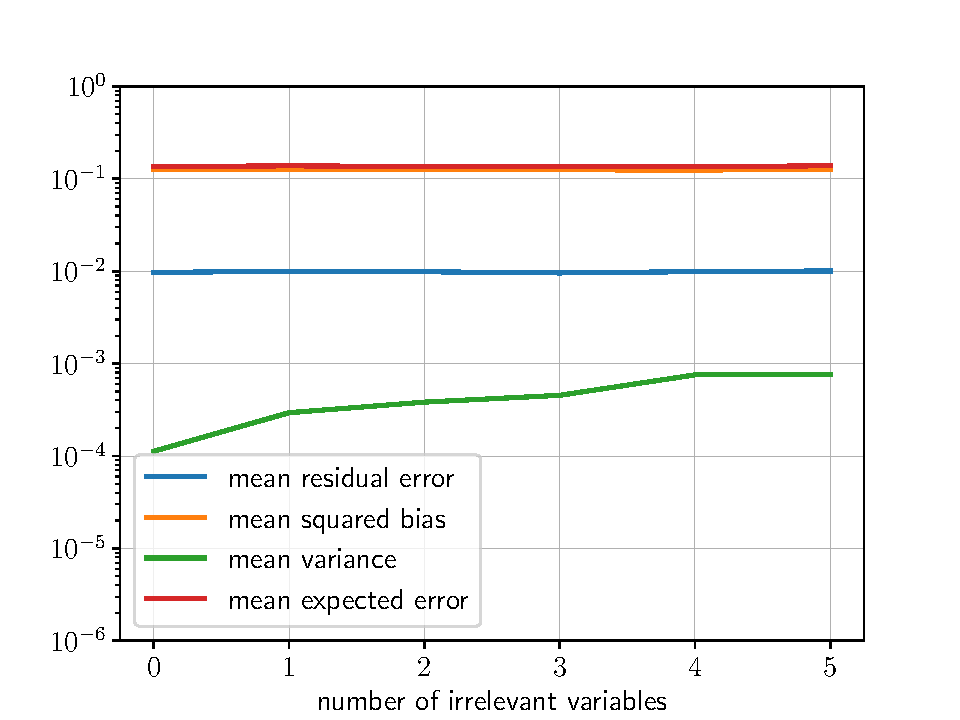
\includegraphics[width=\textwidth]{resources/pdf/Q3e_Ridge_irrelevant_var.pdf}
        \caption{Ridge regression}
    \end{subfigure}
    \begin{subfigure}{0.495\textwidth}
        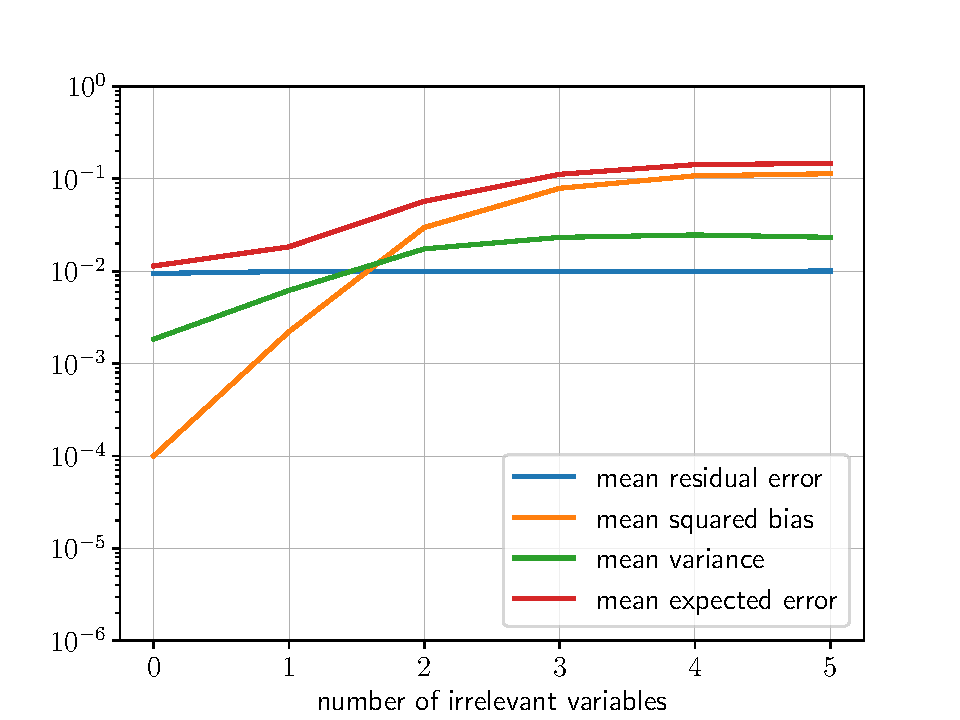
\includegraphics[width=\textwidth]{resources/pdf/Q3e_KNeighborsRegressor_irrelevant_var.pdf}
        \caption{K neighbors regression}
    \end{subfigure}
    \noskipcaption{Mean of the error and its terms as a function of the number of irrelevant variables added to the problem}
\end{figure}
In both cases, as before, the residual error remains constant; it does not depend on the number of irrelevant variables added to the problem.\par
In the linear model, the expected error is always dominated by the squared bias, which remains constant. The reason this is constant may be that we have a lot of samples in our learning sets (1000), and the values of the added variables are randomized between -10 and 10, so their mean will be 0. The regression is therefore not affected by these variables as their contributions will cancel one another.\par
In the non-linear case, the expected error is mainly dominated by the square bias for higher number of irrelevant variables. This may be because adding more variables makes it so that samples that would have been close to one another are more distant, and distant samples may get closer to one another. Indeed, as the values of the added variables are uniform and random, adding more of them means that closer points may grow further apart. The values predicted are therefore worse and the bias increases because the $k$ closest neighbors are not the same as previously, while only $x_r$ should matter in the decision process. This shows that the non-linear model is suitable but that with noise in the features, its quality deteriorates and its results are less and less good. With a high number of irrelevant variables (3 or more), the expected error is the same as the linear model, meaning that the predictions obtained are no longer acceptable.\par
The variance increases with the number of irrelevant variables for both models. For KNN, the predictions for each dataset depend on the particular neighbors, which are modified by the added features (to which we attribute random values), which means that the variance will increase. Indeed, these variables send the samples to different positions in the hyperspace as a result of their values, which are random, and so the variance cannot do anything but increase as two datasets will have otherwise close samples far away depending on the other variables. For the Ridge model, the hypersurface is different for different datasets as it must take into account more random dimensions, the values of the inputs in those varying from one dataset to another, but not too much, as seen in the discussion about the bias.

% Conclusion
\subsubsection*{Conclusion}
The non-linear model (K-nearest neighbors regressor) is clearly preferable to the linear model. This result can be seen throughout the discussions in this section.\par
In order to minimize the expected error of the non linear model, it is therefore necessary to increase the size of the learning set and limit the number of irrelevant variables to a minimum. Increasing the complexity (number of neighbors) does not provide us with a better model, on the contrary.

\end{document}
